\documentclass[10pt,a4paper]{article}
\usepackage[latin1]{inputenc}
\usepackage{amsmath}
\usepackage{amsfonts}
\usepackage{amssymb}
\usepackage{mathtools}
\usepackage{bm}


\newcommand{\vectornorm}[1]{\left\|#1\right\|}

\newcommand{\threepartdef}[6]
{
	\left\{
		\begin{array}{lll}
			#1 & \mbox{for } #2 \\
			#3 & \mbox{for } #4 \\
			#5 & \mbox{for } #6
		\end{array}
	\right.
}

\begin{document}
\title{Semester project\\ Observations}
\author{Espen Johansen Velsvik}
\maketitle

\section*{Choice of regularization parameters}
An experiment for choosing the regularization parameter $\sigma$ was run on the HS algorithm. From Figure \ref{reguHS} it is seen that the choice of $\sigma$ that gives the best result lies somewhere between 0.007 and 0.01. The NE algorithm was then run with $\sigma = 0.007$ for different values of the regularization parameter $\kappa$ to produce Figure \ref{reguNE}. It is seen that the best result comes from choosing $\kappa \approx 1$.

Using the a Sobel filter to approximate the gradients, the maximum value for the term $|\nabla g|^2$ is about $5.5 \cdot 10^5$, which explains why $\kappa$ can be chosen to be relatively large.

\begin{figure}
    \centering
    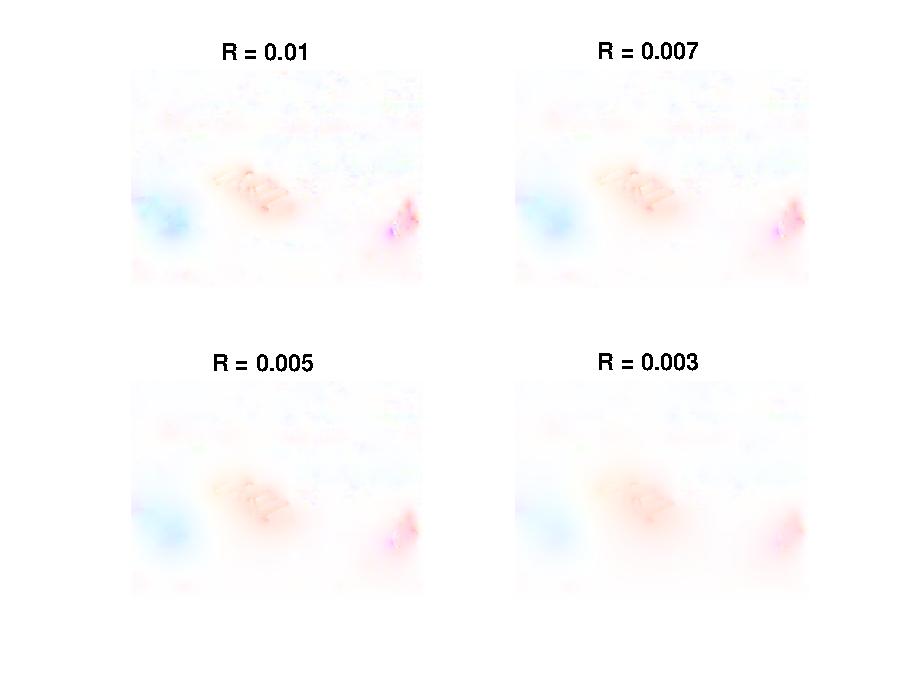
\includegraphics[scale=0.8]{regularizationHS}
    \caption{Different choices for regularization parameter $\sigma$ using the HS algorithm}
    \label{reguHS}
\end{figure}

\begin{figure}
    \centering
    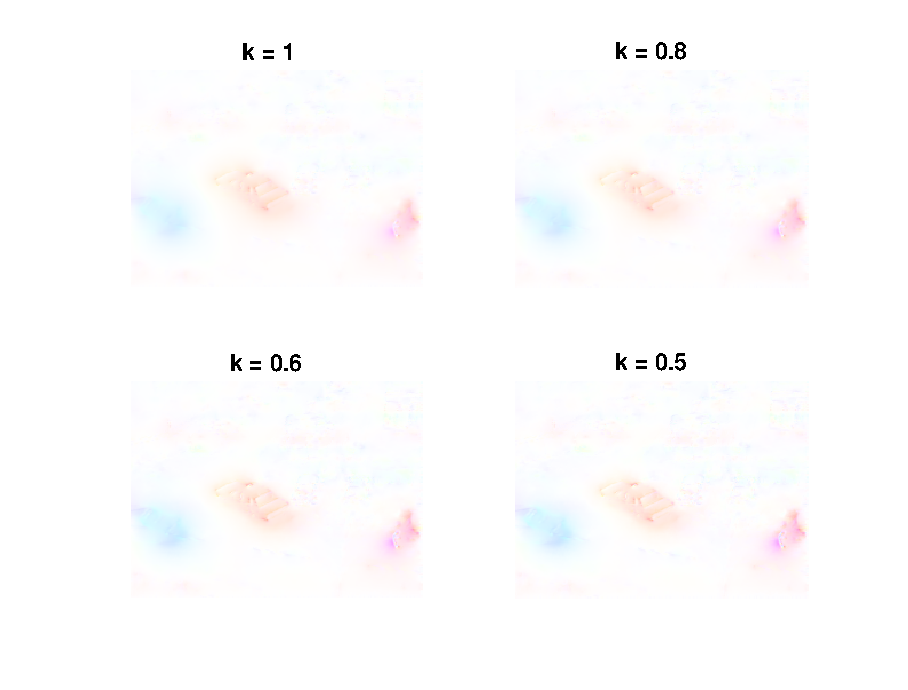
\includegraphics[scale=0.8]{regularizationNE}
    \caption{Different choices for regularization parameter $\kappa$ using the NE algorithm}
    \label{reguNE}
\end{figure}

\end{document}